%%----------------------------------------------------------------------------
%% Presentatie HoGent Bedrijf en Organisatie
%%----------------------------------------------------------------------------
%% Auteur: Bert Van Vreckem [bert.vanvreckem@hogent.be]

\documentclass[notes]{beamer} 

%==============================================================================
% Aanloop
%==============================================================================

%---------- Packages ----------------------------------------------------------

\usepackage{graphicx,multicol}
\usepackage{comment,enumerate,hyperref}
\usepackage{amsmath,amsfonts,amssymb}
\usepackage{tikz}
\usepackage[english]{babel}
\usepackage[utf8]{inputenc}
\usepackage{multirow}
\usepackage{eurosym}
\usepackage{listings}
\usepackage[T1]{fontenc}
\usepackage{lmodern}
\usepackage{textcomp}
\usepackage{framed}
\usepackage{wrapfig}
\usepackage{pgfpages}



%---------- Configuratie ------------------------------------------------------

\usetikzlibrary{arrows,shapes,backgrounds,positioning,shadows}

\usetheme{hogent}

%---------- Commando-definities -----------------------------------------------

\newcommand{\tabitem}{~~\llap{\textbullet}~~}

%---------- Info over de presentatie ------------------------------------------

\title[Intro]{Creative Thinking}
\author{Jens Buysse}
\date{\today}

%==============================================================================
% Inhoud presentatie
%==============================================================================

\begin{document}

%---------- Front matter ------------------------------------------------------

% Dia met het HoGent logo
\HoGentLogo

% Titeldia met faculteitslogo
\titleframe

%---------- Inhoud ------------------------------------------------------------

\begin{frame}
  \frametitle{Inhoud}

  \tableofcontents
\end{frame}

\section{What is creative thinking}

\sectionframe{\begin{center}
		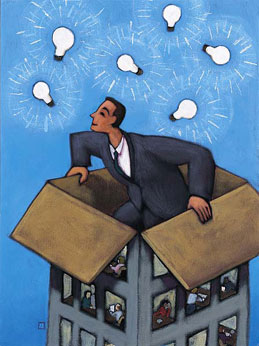
\includegraphics[height=0.6\textheight]{img/intro.jpg}
\end{center}}

\begin{frame}{What is thinking?}
	\begin{center}
		\begin{figure}
			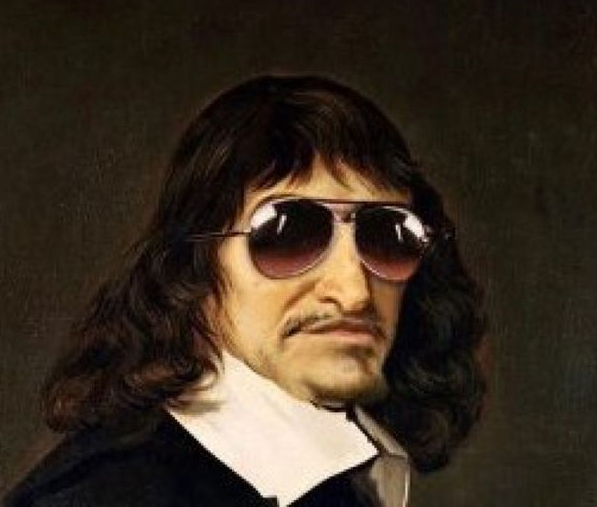
\includegraphics[height=0.6 \textheight]{img/rene.jpg}
		\end{figure}
	\end{center}
\note{Descartes tries to give a definition of "thought" in principle I.9. By "thought" he tells us, he means to refer to anything marked by awareness or consciousness. This does not just include reasoning or other such intellectual activities but also imagining, sensing, willing, believing, doubting, hoping, dreading, and all other mental operations.}
\end{frame}


\begin{frame}{What is thinking?}
	\begin{figure}
		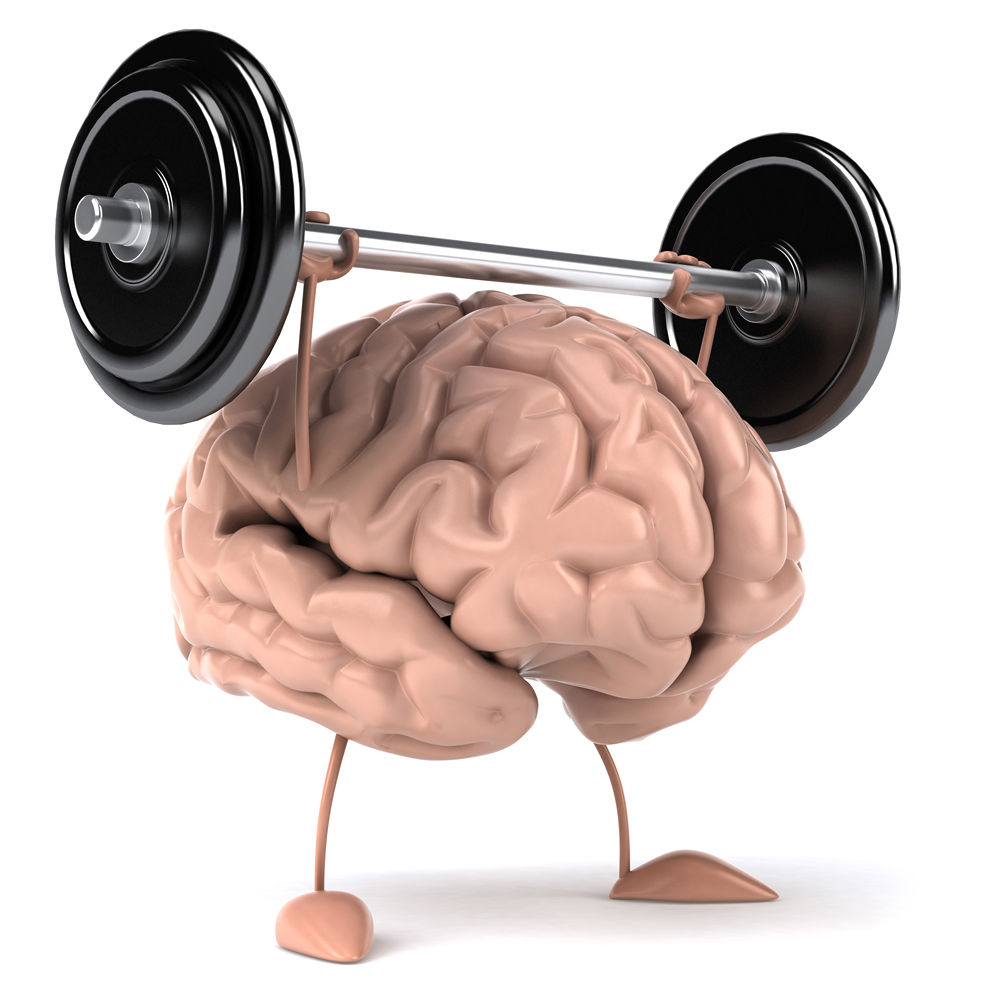
\includegraphics[height=0.6\textheight]{img/brain.jpg}
	\end{figure}
\note{Your brain is made of approximately 100 billion nerve cells, called neurons. Neurons have the amazing ability to gather and transmit electrochemical signals (up to several feet or a few meters) and send messages to each other. Dendrites or nerve endings. These small, branchlike projections of the cell make connections to other cells and allow the neuron to talk with other cells or perceive the environment. Dendrites can be located on one or both ends of a cell.}
\end{frame}

\begin{frame}{What is thinking?}
	\href{http://www.youtube.com/watch?v=BGPGknpq3e0}{Is \underline{this} an example of thinking?}
\end{frame}

\begin{frame}{Excercise}
	\brightbox{Take a sheet of paper and draw an \textcolor{HoGentAccent6}{alien}}
	\note{Most of the studenst will have drawn a default alien with arms and legs and eyes. But why not a blob, or a dot, or just a line}
\end{frame}


\begin{frame}{What is \textcolor{HoGentAccent6}{creative} thinking?}
	\begin{figure}
		\includegraphics[width=10cm]{img/babydriving}
	\end{figure}
\end{frame}

\begin{frame}{What is \textcolor{HoGentAccent6}{creative} thinking?}
	\begin{figure}
		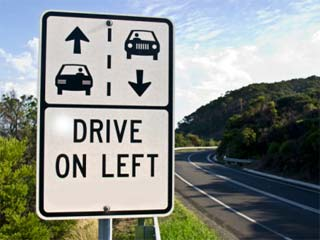
\includegraphics[width=8cm]{img/drive.jpg}
	\end{figure}
\end{frame}

\begin{frame}{What is \textcolor{HoGentAccent6}{creative} thinking?}
	\begin{itemize}
		\item Experience is the sum of patterns.
		\item Patterns which we have created througout or life
		\item \textcolor{HoGentAccent1}{Creative thinking} is trying to break these patterns which we are so accustomed to. 
	\end{itemize}

\begin{center}
	\begin{figure}
		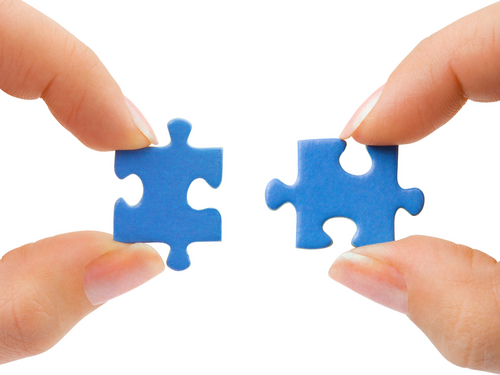
\includegraphics[width=5cm]{img/puzzel.jpg}
	\end{figure}
\end{center}
\end{frame}

\begin{frame}{Excercise}
	\begin{itemize}
		\item There is blood on the ceiling. There has been no murder of killing or accident. Nobody has played a trick on me. Can you suggest an explanation. 
	\end{itemize}

\note{A mosquito bit me, landed on the ceiling and and I swatted it.}
\end{frame}

\begin{frame}{Excercise}
	\begin{itemize}
		\item There is a flash of light and a man dies. The man is not killed by any other person and he does not die of an illness like a heart attack \dots It is not suicide. Can you suggest an explanation?
	\end{itemize}
	
	\note{The man is a lion tamer, posing for a photo with the lion. Somebody took a picture and the lion reacted badly, so he gets mauled}
\end{frame} 

\begin{frame}{Excercise}
	\begin{itemize}
		\item An ordinary American Citizen with no passport on him visits over thirthy oreign countries in one day. He is welcomed in each country and leaves each one of his own accord?
	\end{itemize}
	
	\note{He is a mail courier who delivers packages to different foreign embassies in the embassies. The land of an embassy belongs to the country of the embassy, not the united states.}
\end{frame}

\section{Attitudes towards Creative Thinking}

\sectionframe{\begin{center}
		
\includegraphics[width=0.8\textwidth]{img/attitude.jpg}
\end{center}}	

{ % all template changes are local to this group.
	\setbeamertemplate{navigation symbols}{}
	\begin{frame}[plain]
		\begin{tikzpicture}[remember picture,overlay]
		\node[at=(current page.center)] {
			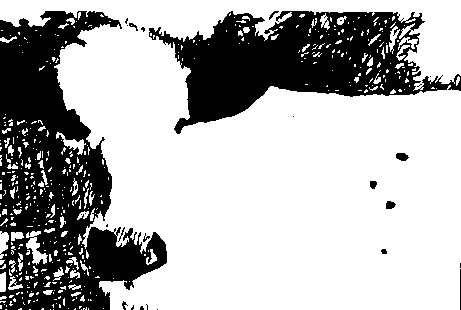
\includegraphics[width=\paperwidth]{img/cow.png}
		};
		\end{tikzpicture}
	\end{frame}
}

{ % all template changes are local to this group.
	\setbeamertemplate{navigation symbols}{}
	\begin{frame}[plain]
		\begin{tikzpicture}[remember picture,overlay]
		\node[at=(current page.center)] {
			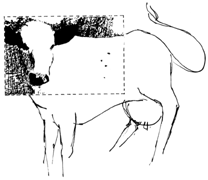
\includegraphics[width=\paperwidth]{img/cow2.png}
		};
		\end{tikzpicture}
	\end{frame}
}

\begin{frame}{Creative perception}
	\begin{itemize}
		\item \textcolor{HoGentAccent1}{Creative perception} is to recognize your own \textcolor{HoGentAccent1}{dominant} view and to be capable of finding alternative perceptions
	\end{itemize}
\pause
\begin{columns}
	\begin{column}{0.5\textwidth}
		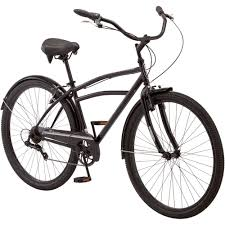
\includegraphics[width = 0.9 \textwidth]{img/bike.jpeg}
	\end{column}
	\begin{column}{0.5\textwidth}
	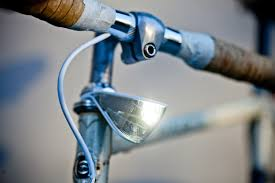
\includegraphics[width = \textwidth]{img/light.jpeg}
\end{column}
\end{columns}
\note{Bikes were used during the war as a light source and not only a mode of transport}
\end{frame}

{ % all template changes are local to this group.
	\setbeamertemplate{navigation symbols}{}
	\begin{frame}[plain]
		\begin{tikzpicture}[remember picture,overlay]
		\node[at=(current page.center)] {
			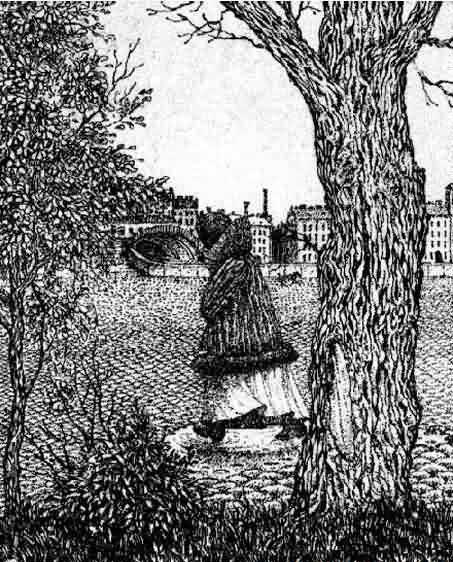
\includegraphics[height=\paperheight]{img/illusion1.png}
		};
		\end{tikzpicture}
	\end{frame}
}

{ % all template changes are local to this group.
	\setbeamertemplate{navigation symbols}{}
	\begin{frame}[plain]
		\begin{tikzpicture}[remember picture,overlay]
		\node[at=(current page.center)] {
			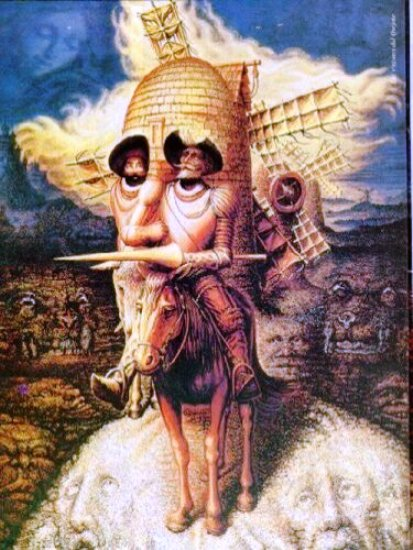
\includegraphics[height=\paperheight]{img/don.png}
		};
		\end{tikzpicture}
	\end{frame}
}

{ % all template changes are local to this group.
	\setbeamertemplate{navigation symbols}{}
	\begin{frame}[plain]
		\begin{tikzpicture}[remember picture,overlay]
		\node[at=(current page.center)] {
			
\includegraphics[height=\paperheight]{img/liar.png}
		};
		\end{tikzpicture}
	\end{frame}
}


\begin{frame}{Postpone judgement}
	\begin{itemize}
		\item We judge by different levels
		\begin{itemize}
			\item Unconsciously: just do not listen
			\item You are listening, but you decide if you pay attention
			\item You are careful but you do not use the information
		\end{itemize}
		Unconsciously: just do not listen
	\end{itemize}
\end{frame}

\begin{frame}{Postpone judgement}
	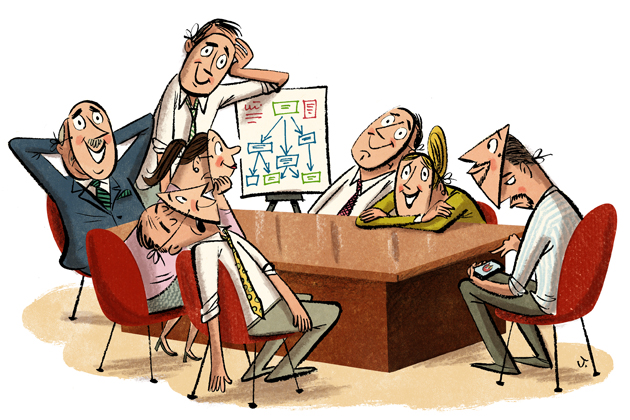
\includegraphics[width=\textwidth]{img/group.jpg}
\end{frame}

\begin{frame}{Postpone judgement: exercise}
	\brightbox{Think of something that you like very much. TV program, favorite chips \dots Now you have to think of as many bad things as possible - no matter how weird. Try turning these things into something positive now.}
\end{frame}

\begin{frame}{Association}
	\begin{itemize}
		\item In association, different things are linked to each other in mind.
	\end{itemize}
	\begin{columns}
		\begin{column}{0.3\textwidth}
			\begin{center}
				Lemon
			\end{center}
			
\includegraphics[width=\textwidth]{img/lemon.png}
		\end{column} \pause
			\begin{column}{0.3\textwidth}
				\begin{center}
					Sour
				\end{center}
		
\includegraphics[width=\textwidth]{img/sour.jpg}
	\end{column} \pause
			\begin{column}{0.3\textwidth}
				\begin{center}
					Acid
				\end{center}
	
\includegraphics[width=\textwidth]{img/acid.jpeg}
\end{column}
	\end{columns}
\end{frame}

\begin{frame}{Associations}
	One popular answer to why fire trucks are red goes something like this:
	\brightbox{“Because they have eight wheels and four people on them, and four plus eight makes twelve, and there are twelve inches in a foot, and one foot is a ruler, and Queen Elizabeth was a ruler, and Queen Elizabeth was also a ship, and the ship sailed the seas, and there were fish in the seas, and fish have fins, and the Finns fought the Russians, and the Russians are red, and fire trucks are always “Russian" around, so that's why fire trucks are red!"}
\end{frame}

\begin{frame}{Association exercises}
	\begin{itemize}
		\item Normal association
		\item Association starting with pencil and ending with Jupiter
		\item Same as above but try to invent a story with the words found
		\item \dots
	\end{itemize}
Continue when you are facing difficulties $\rightarrow$ then it becomes interesting!
\end{frame}

\begin{frame}
	\begin{center}
		\Huge A E I F U 
	\end{center}
\note{Questions is which letter does not fit the series. Of course there are multiple solutions, the more you look at the letters. }
\end{frame}

\begin{frame}{Diverge}
	Once you have an idea or a solution, it's important that you thoroughly understand and diverge the solution. For example, use association.
\end{frame}

{ % all template changes are local to this group.
	\setbeamertemplate{navigation symbols}{}
	\begin{frame}[plain]
		\begin{tikzpicture}[remember picture,overlay]
		\node[at=(current page.center)] {
			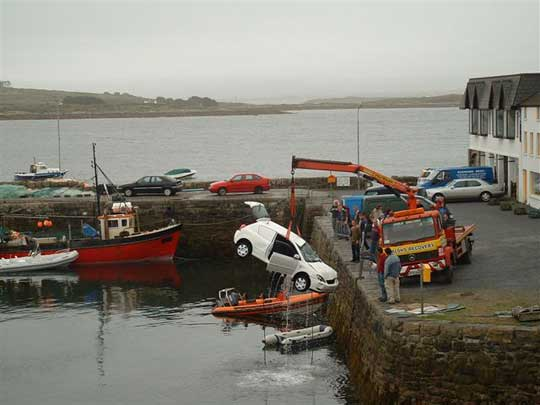
\includegraphics[height=\paperheight]{img/car1.png}
		};
		\end{tikzpicture}
	\end{frame}
}

{ % all template changes are local to this group.
	\setbeamertemplate{navigation symbols}{}
	\begin{frame}[plain]
		\begin{tikzpicture}[remember picture,overlay]
		\node[at=(current page.center)] {
			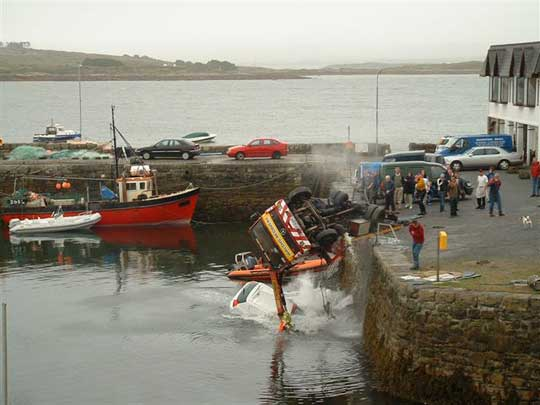
\includegraphics[height=\paperheight]{img/car2.png}
		};
		\end{tikzpicture}
	\end{frame}
}

{ % all template changes are local to this group.
	\setbeamertemplate{navigation symbols}{}
	\begin{frame}[plain]
		\begin{tikzpicture}[remember picture,overlay]
		\node[at=(current page.center)] {
			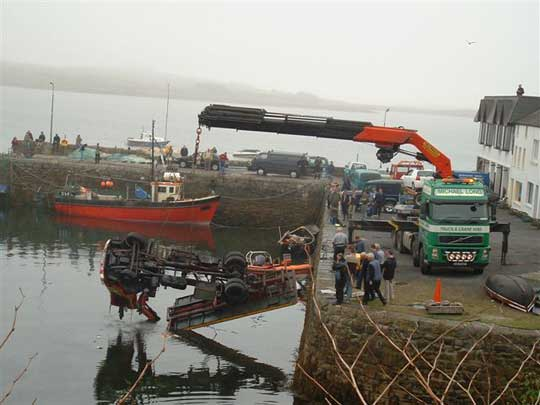
\includegraphics[height=\paperheight]{img/car3.png}
		};
		\end{tikzpicture}
	\end{frame}
}

{ % all template changes are local to this group.
	\setbeamertemplate{navigation symbols}{}
	\begin{frame}[plain]
		\begin{tikzpicture}[remember picture,overlay]
		\node[at=(current page.center)] {
			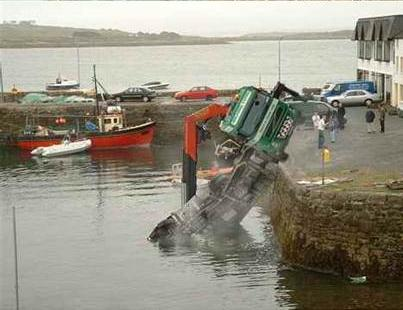
\includegraphics[height=\paperheight]{img/car4.png}
		};
		\end{tikzpicture}
	\end{frame}
}
\section{Creative techniques}
\sectionframe{}

\begin{frame}{The creative proces}
\begin{enumerate}
	\item Start and prepare
	
	\item Expiration phase (diverge)
	
	\item Reconcile (converge)
\end{enumerate}
\end{frame}

\begin{frame}{Start \& preparation}
	\begin{itemize}
		\item Make a question or query in 1 sentence.
		
		\item Do not formulate broadly and maintain concrete focus
		
		\item The problem holder must be in the formulation
		
		\item Start the question with "How" or "Create"
		
		\item Overformulate the question
	\end{itemize}
\end{frame}

\begin{frame}{Direct analog}
	Find an analog: an object / animal / \dots that satisfies 1 of the following properties.
	\begin{itemize}
			\item As far as possible from the context of problem statement.
		\item Inspiring
		
	\end{itemize}

	
	Examples are: Countries (China), Animals (Squid) \dots
	
	Write down characteristics of it and use it as a starting point to solve our problem.
\end{frame}

\begin{frame}{Analog: superhero}
	\begin{itemize}
		\item Find a superhero that interests you:
		
		\item Examples are: zorro, superman \dots
		
		\item How would this superhero solve it?
		
		\item Find answers in concrete solutions.
	\end{itemize}
\end{frame}

\begin{frame}{Personal analogy}
	\begin{enumerate}
		\item Choose an important object from the question statement.
		
		
		\item Describe how you would feel if you were that object in that context.
		How would you react? How would you solve it?
		
		\item Solve solution in concrete solutions.
	\end{enumerate}
\end{frame}

{ % all template changes are local to this group.
	\setbeamertemplate{navigation symbols}{}
	\begin{frame}[plain]
		\begin{tikzpicture}[remember picture,overlay]
		\node[at=(current page.center)] {
			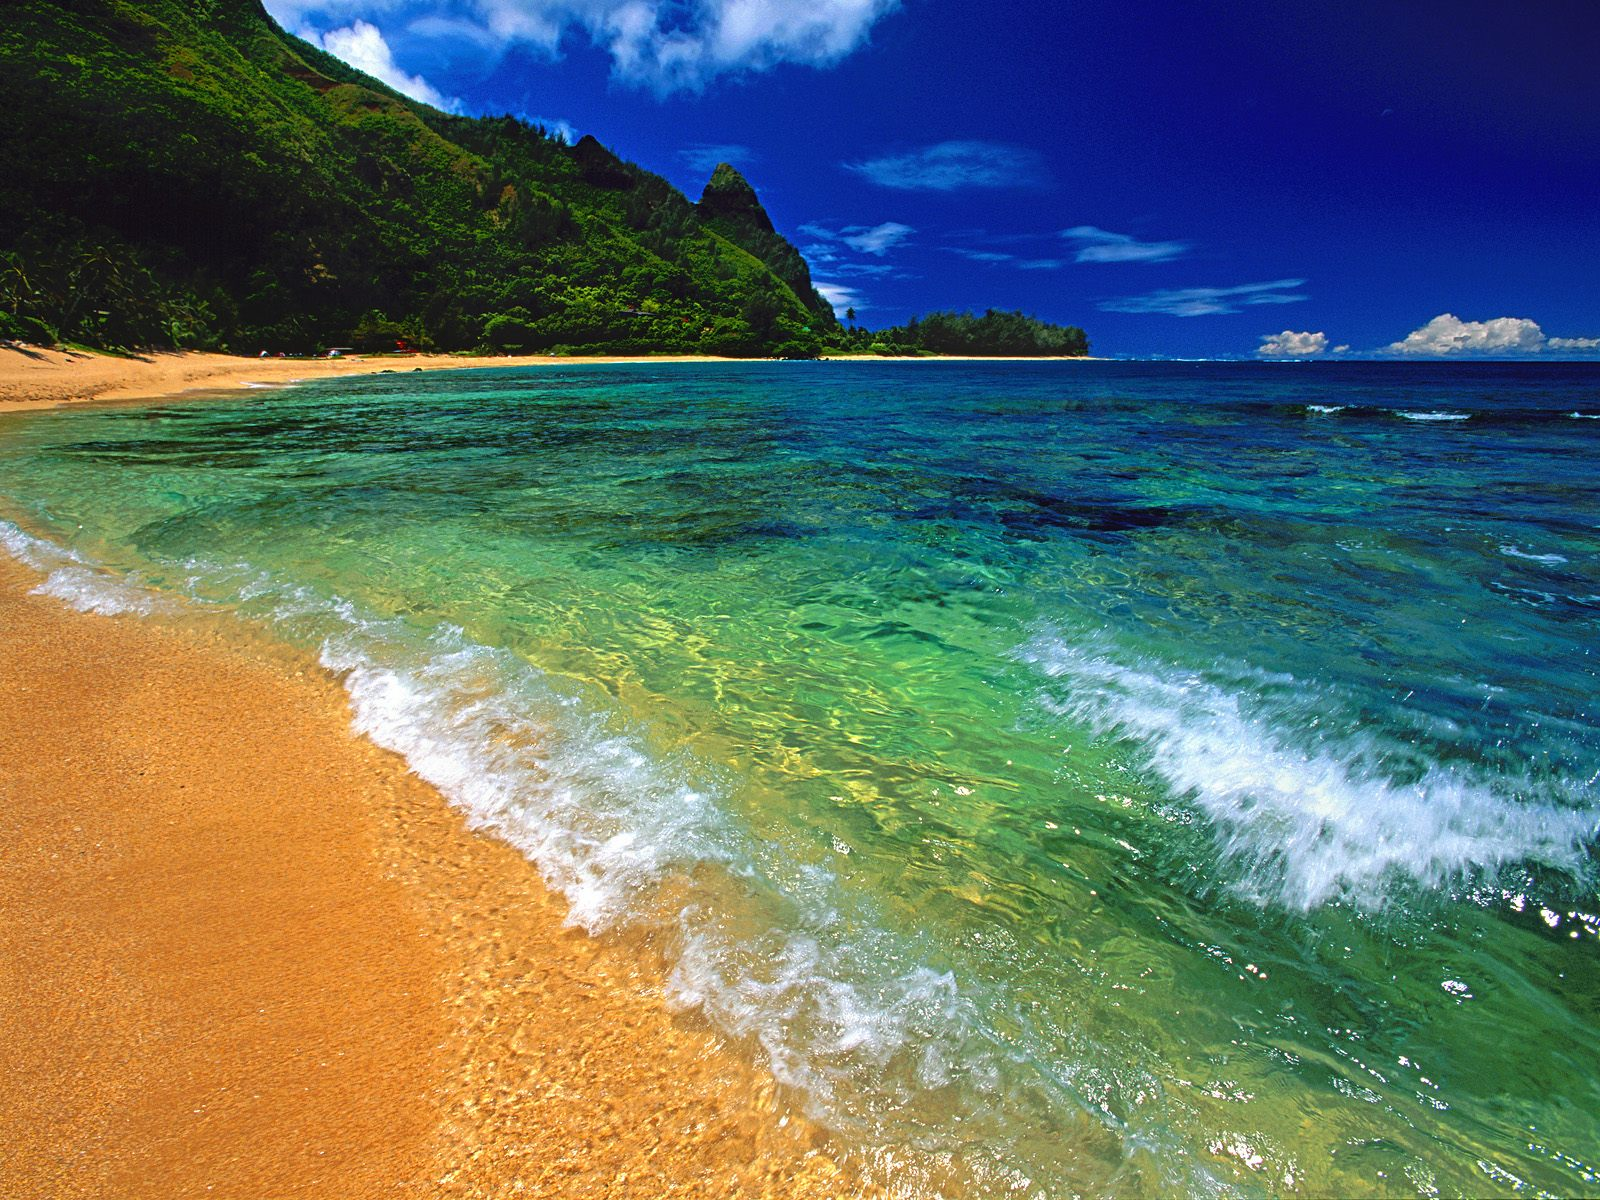
\includegraphics[height=\paperheight]{img/beach.jpg}
		};
		\end{tikzpicture}
	\end{frame}
}

\begin{frame}{Alphabet brainstorm}
	\begin{itemize}
		\item 
		Choose for each letter of the alphabet a possible solution ...
		\begin{enumerate}[A]
			\item \dots
			\item \dots
			\item \dots
		\end{enumerate}		
		
		\item Make possible solution in concrete solutions
	\end{itemize}
\end{frame}

\begin{frame}{Converge}
\begin{center}
		\begin{tikzpicture}
	\draw[step=1cm,gray,very thin] (-2,-2) grid (6,6);
	
	\filldraw[fill=HoGentAccent1, draw=black] (-2,-2) rectangle (2,2) node[ inner sep=5pt, pos=0.5,anchor=north] {easy \& normal};
	\filldraw[fill=HoGentAccent2, draw=black] (6,2) rectangle (2,-2) node[ inner sep=5pt, pos=0.5,anchor=north] {easy \& original};
	\filldraw[fill=HoGentAccent6, draw=black] (2,2) rectangle (6,6)node[ inner sep=5pt, pos=0.5,anchor=north] {impossible \& original};
		\draw[thick,->] (-2,-2) -- (6,-2) node[anchor=north west] {originality};
	\draw[thick,->] (-2,-2) -- (-2,6) node[anchor=north west] {difficulty};
	\end{tikzpicture}
\end{center}
\end{frame}

\begin{frame}{Converge \& Combine}
		\begin{columns}
		\begin{column}{0.3\textwidth}
			\begin{center}
				Tape
			\end{center}
			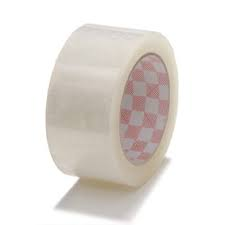
\includegraphics[width=\textwidth]{img/tape.png}
		\end{column} \pause
		\begin{column}{0.3\textwidth}
			\begin{center}
				Scissor
			\end{center}
			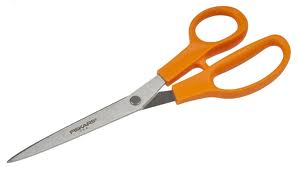
\includegraphics[width=\textwidth]{img/scissor.png}
		\end{column} \pause
		\begin{column}{0.3\textwidth}
			\begin{center}
				Tape deck
			\end{center}
			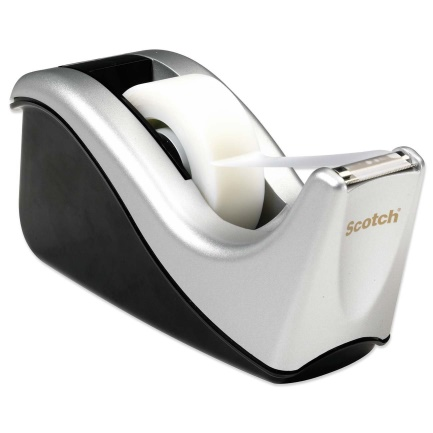
\includegraphics[width=\textwidth]{img/tapedeck.jpg}
		\end{column}
	\end{columns}

\end{frame}

\begin{frame}{Combine yellow and red ideas}
	Birthday party in the forest
	$+$
	A theme party
	$+$
	Magic game
	$=$
	
	\brightbox{We celebrate Mum's birthday in the
	the forest with a magic theme!}
\end{frame}

\begin{frame}{Combine yellow and red ideas}
Everyone takes a strange object
$+$
Everybody takes something to sit up on


$=$


	\brightbox{Everyone takes something to sit up that is not a chair}
\end{frame}

\section{Conclusions \& lessons learned}
\sectionframe{\begin{center}
		
\includegraphics[height=0.6\textwidth]{img/piet.jpg}
\end{center}}
\begin{frame}{Conclusions \& lessons learned}
	
	\brightbox{Creative thinking is the art of breaking patterns}
\begin{itemize}
	\item Skills and attitudes
	\item Creative perception
	\item Deferral of judgment
	\item Associate
	\item Diverge
\end{itemize}
\brightbox{The creative process consists of three phases}
 \begin{enumerate}
 \item Starting phase
 \item Diverge
 \item Converge
 \end{enumerate}
Results in COCD
$\rightarrow$ Combine fun ideas!
	
\end{frame}



%---------- Back matter -------------------------------------------------------

\end{document}
